\documentclass{article}
% Chinese
% \documentclass[UTF8, nofonts, mathptmx, 12pt, onecolumn]{article}
% \usepackage{xeCJK}
% \setCJKmainfont{SimSun}
\usepackage{amsmath}
\usepackage{amsfonts}
\usepackage{amssymb}
\usepackage{wasysym}
% \usepackage{ctex}
\usepackage{graphicx}
\usepackage{float}
\usepackage{geometry}
\geometry{a4paper,scale=0.8}
\usepackage{caption}
\usepackage{subcaption}
% \newcommand{\oiint}{\mathop{{\int\!\!\!\!\!\int}\mkern-21mu \bigcirc} {}}
\newcommand*{\dif}{\mathop{}\!\mathrm{d}}
\newcommand*{\md}{\mathop{}\!\mathrm{d}}
\newcommand*{\me}{\mathrm{e}}

% \usepackage{parskip}
% \setlength{\parindent}{0cm}

\usepackage{bm}
\let\Oldmathbf\mathbf
\renewcommand{\mathbf}[1]{\boldsymbol{\Oldmathbf{#1}}}
\let\eqnarray\align

\author{Xiping Hu}
\usepackage{authblk}
\author{Xiping Hu}
\affil{https://hxp.plus/}
\title{Homework for Chapter 5}

\begin{document}
\maketitle

\begin{figure}[H]
  \centering
  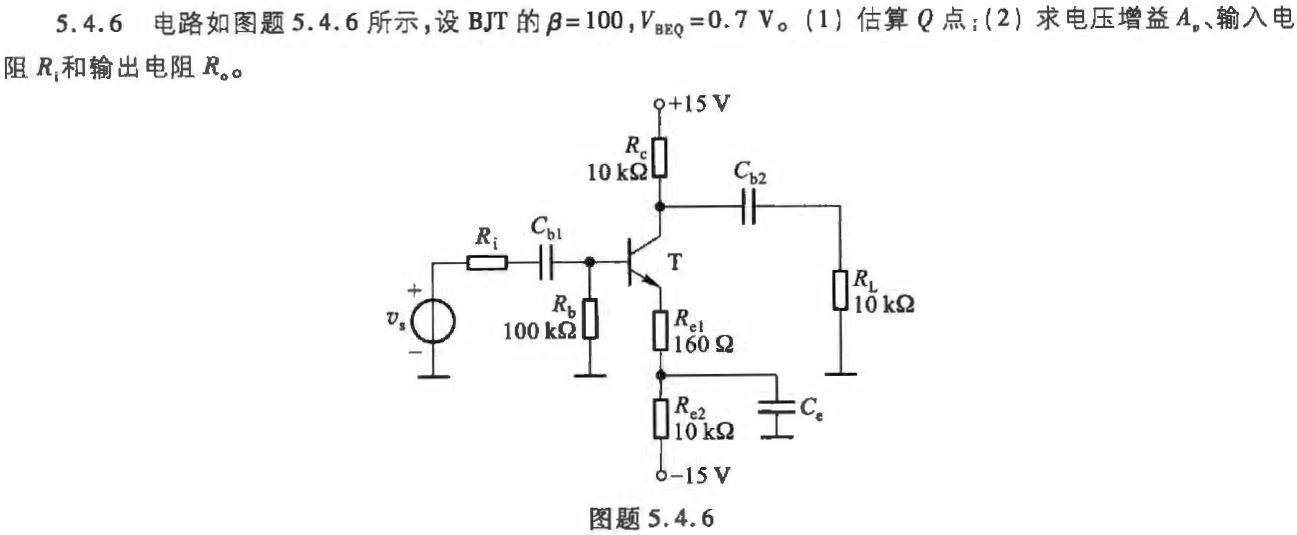
\includegraphics[width=\linewidth]{figures/Problem546}
  \label{fig:}
\end{figure}

\begin{figure}[H]
  \centering
  \begin{subfigure}{.3\textwidth}
    \centering
    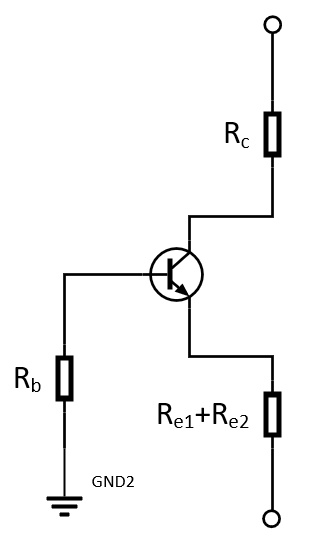
\includegraphics[width=0.7\linewidth]{figures/Problem5461}
    \label{fig:}
  \end{subfigure}%
  \begin{subfigure}{.8\textwidth}
    \centering
    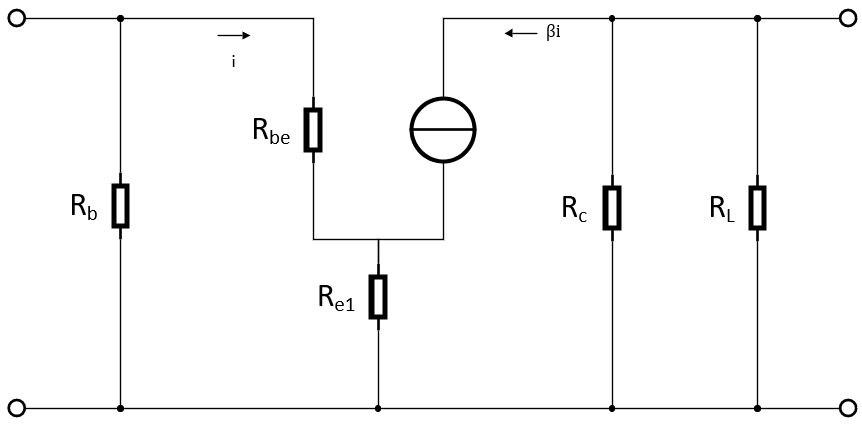
\includegraphics[width=0.8\linewidth]{figures/Problem5462}
    \label{fig:}
  \end{subfigure}
  \label{fig:}
\end{figure}

\paragraph{Problem 1}

\begin{equation*}
  \begin{aligned}
    I_{BQ} = \dfrac{\left( 15 - 0.7 \right) \mathrm{V}}{R_b + \left( 1 + \beta \right) \left( R_{e1} + R_{e2} \right)} = 12.7 \  \mathrm{\mu A}
  \end{aligned}
\end{equation*}

\begin{equation*}
  \begin{aligned}
    V_{CEQ} = 30 - \beta I_{BQ} \left( R_C + R_{e1} + R_{e2} \right) = 4.4 \  \mathrm{V}
  \end{aligned}
\end{equation*}

\paragraph{Problem 2}

\begin{equation*}
  \begin{aligned}
    r_{be} = 200 \  \mathrm{\Omega} + \left( 1 + \beta \right) \dfrac{26 \  \mathrm{mV}}{I_{EQ} \left( \mathrm{mA} \right)} = 2.27 \  \mathrm{k \Omega}
  \end{aligned}
\end{equation*}

\begin{equation*}
  \begin{aligned}
    A_v = - \dfrac{\beta \left( R_c \parallel R_L \right)}{r_{be} + \left( 1 + \beta \right) R_{e1}} = - 27.13
  \end{aligned}
\end{equation*}

\begin{equation*}
  \begin{aligned}
    R_i = R_b \parallel \left[ r_{be} + \left( 1 + \beta \right) R_{e1} \right] = 15.56 \  \mathrm{k \Omega}
  \end{aligned}
\end{equation*}

\begin{equation*}
  \begin{aligned}
    R_o = R_L = 10 \  \mathrm{k \Omega}
  \end{aligned}
\end{equation*}

\end{document}